

This section contains the project analysis done using Alloy.\\
\subsection{Introduction}
The alloy model is focused on the main entities and rules of SS:
\begin{itemize}
	\item User-made reports
	\item Main actors
	\item Rules regarding user-made reports
	\item Rules regarding police intervention
	\item Rules regarding data mining rights
\end{itemize}
While, on the other hand, cross-database interactions have not been modeled and the relation between area and violation has not been modeled in its entirety, as the rules about how to assign a violation to an area are missing.\\  
Please note that the violation types are actually more than the 2 reported in the alloy model, but in order to keep the model simple I have only represented ExpiredParking and UnlawfulParking.\\
\\
\newpage
\subsection{Signatures}
\begin{figure}[h!]
	\centering
	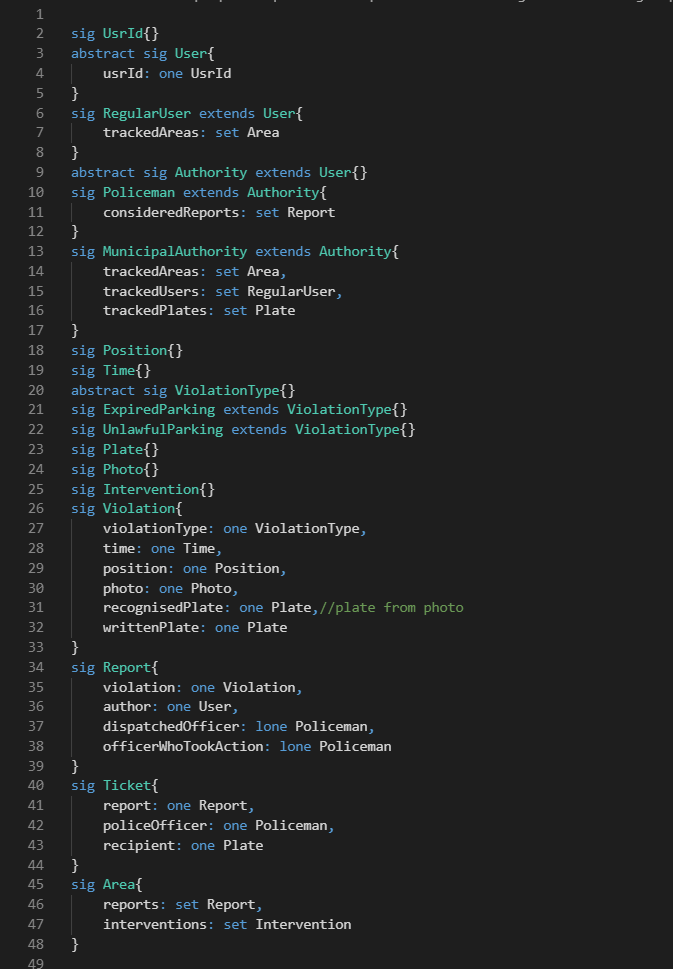
\includegraphics[scale=0.85 ]{Images/Signatures_1-2}
	\caption{Alloy model signatures}
\end{figure}
\newpage
\subsection{Facts}
\begin{figure}[h!]
	\centering
	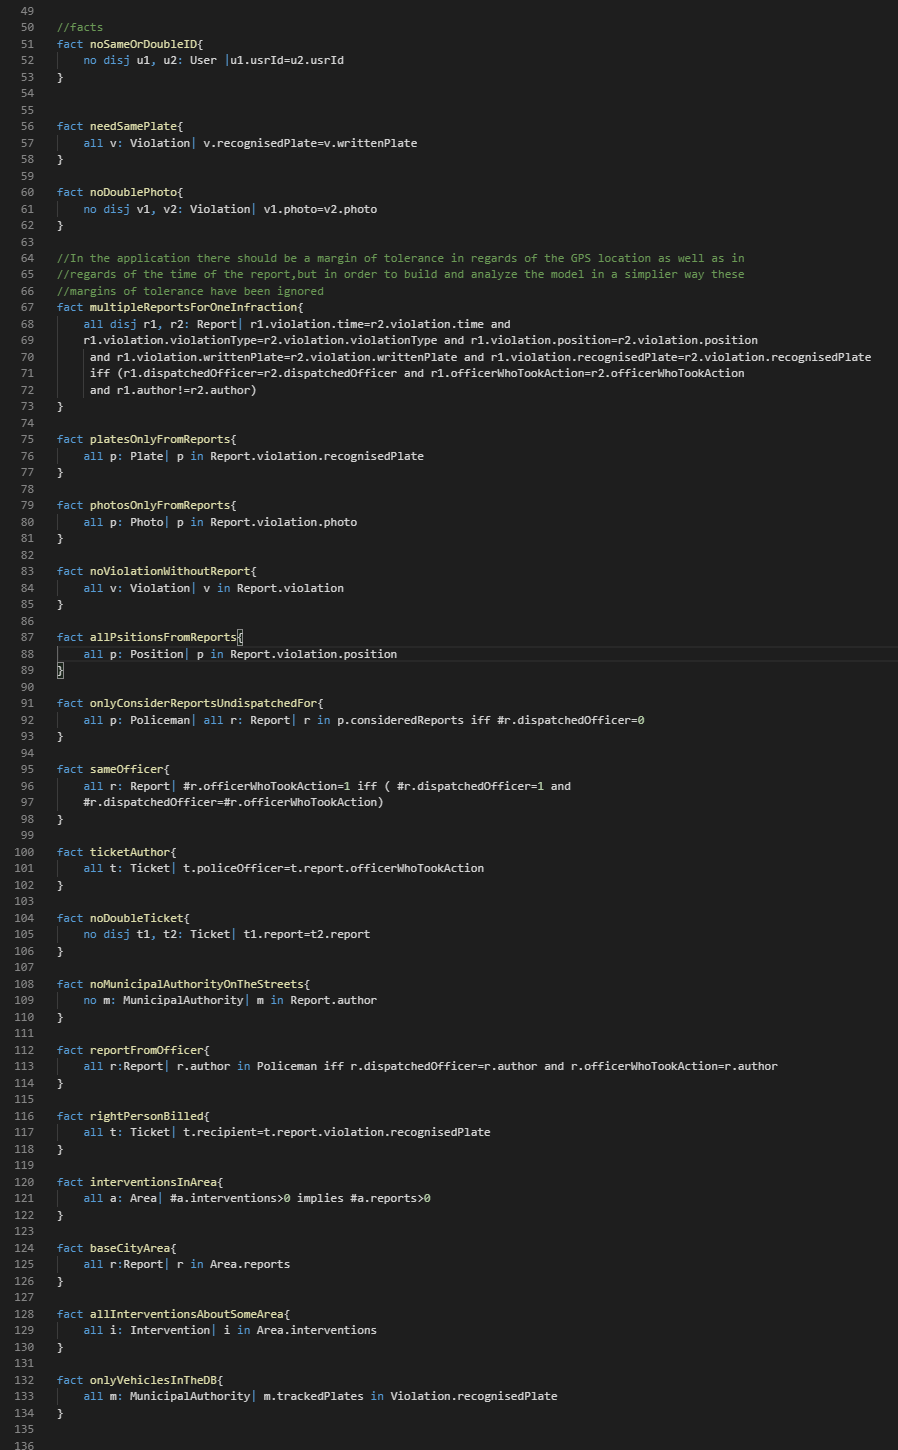
\includegraphics[scale=0.58]{Images/Facts_1-2}
	\caption{Alloy model facts}
\end{figure}
\newpage
\subsection{Assertions and world}
\begin{figure}[h!]
	\centering
	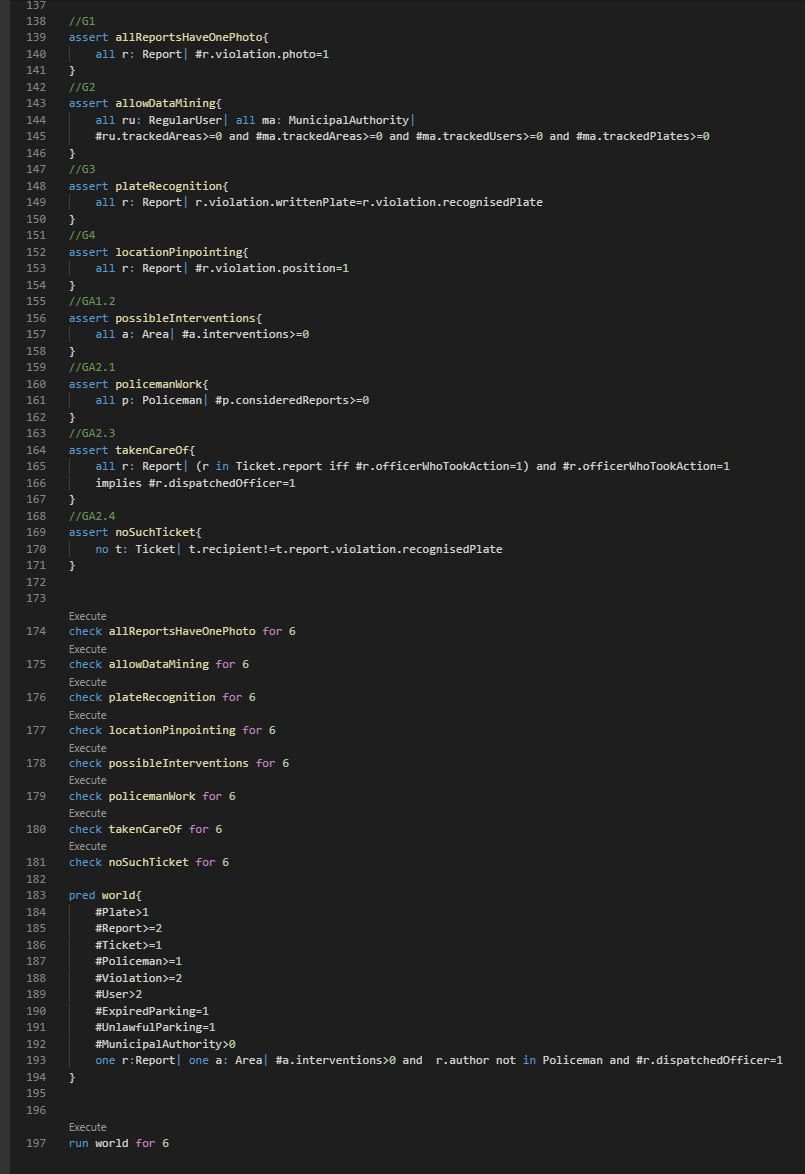
\includegraphics[scale=0.70]{Images/Assertions_and_world_1-2}
	\caption{Alloy model assertions and world declaration}
\end{figure}
\newpage
\subsection{Results}
\subsubsection{Checks on assertions}
\begin{figure}[h!]
	\centering
	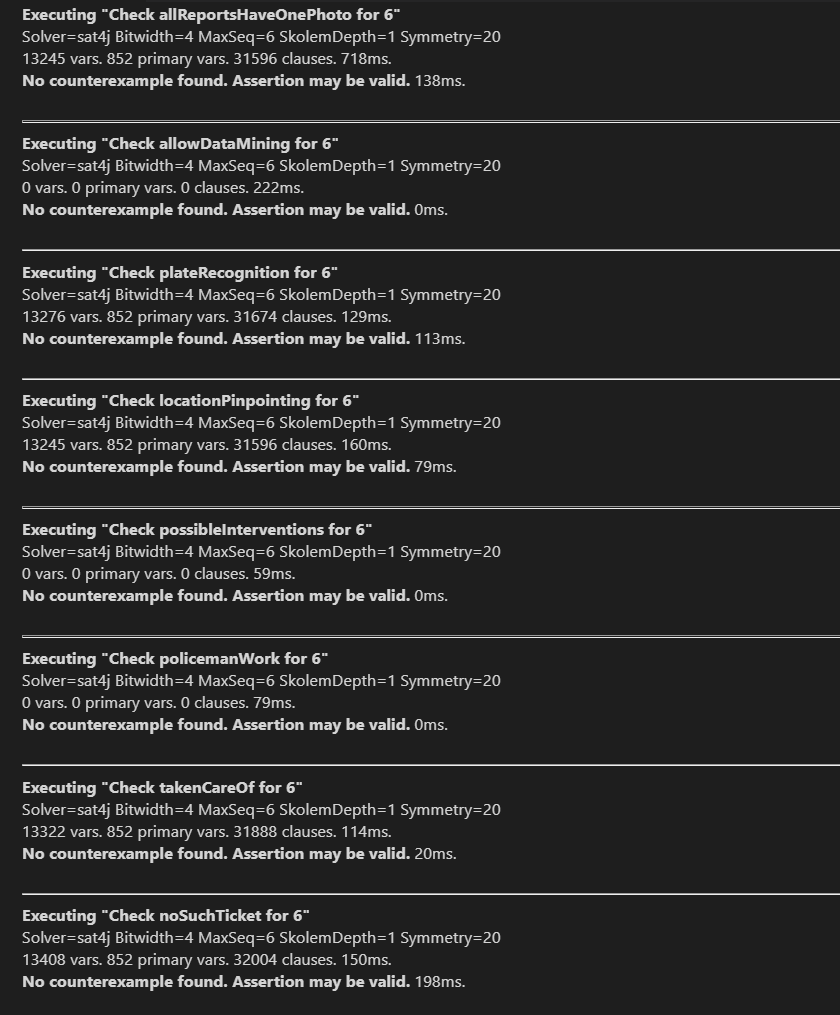
\includegraphics[scale=0.70]{Images/Assertions_result}
	\caption{Results of the checks on the assertions}
\end{figure}
\newpage
\subsubsection{World generated}
\begin{figure}[h!]
	\centering
	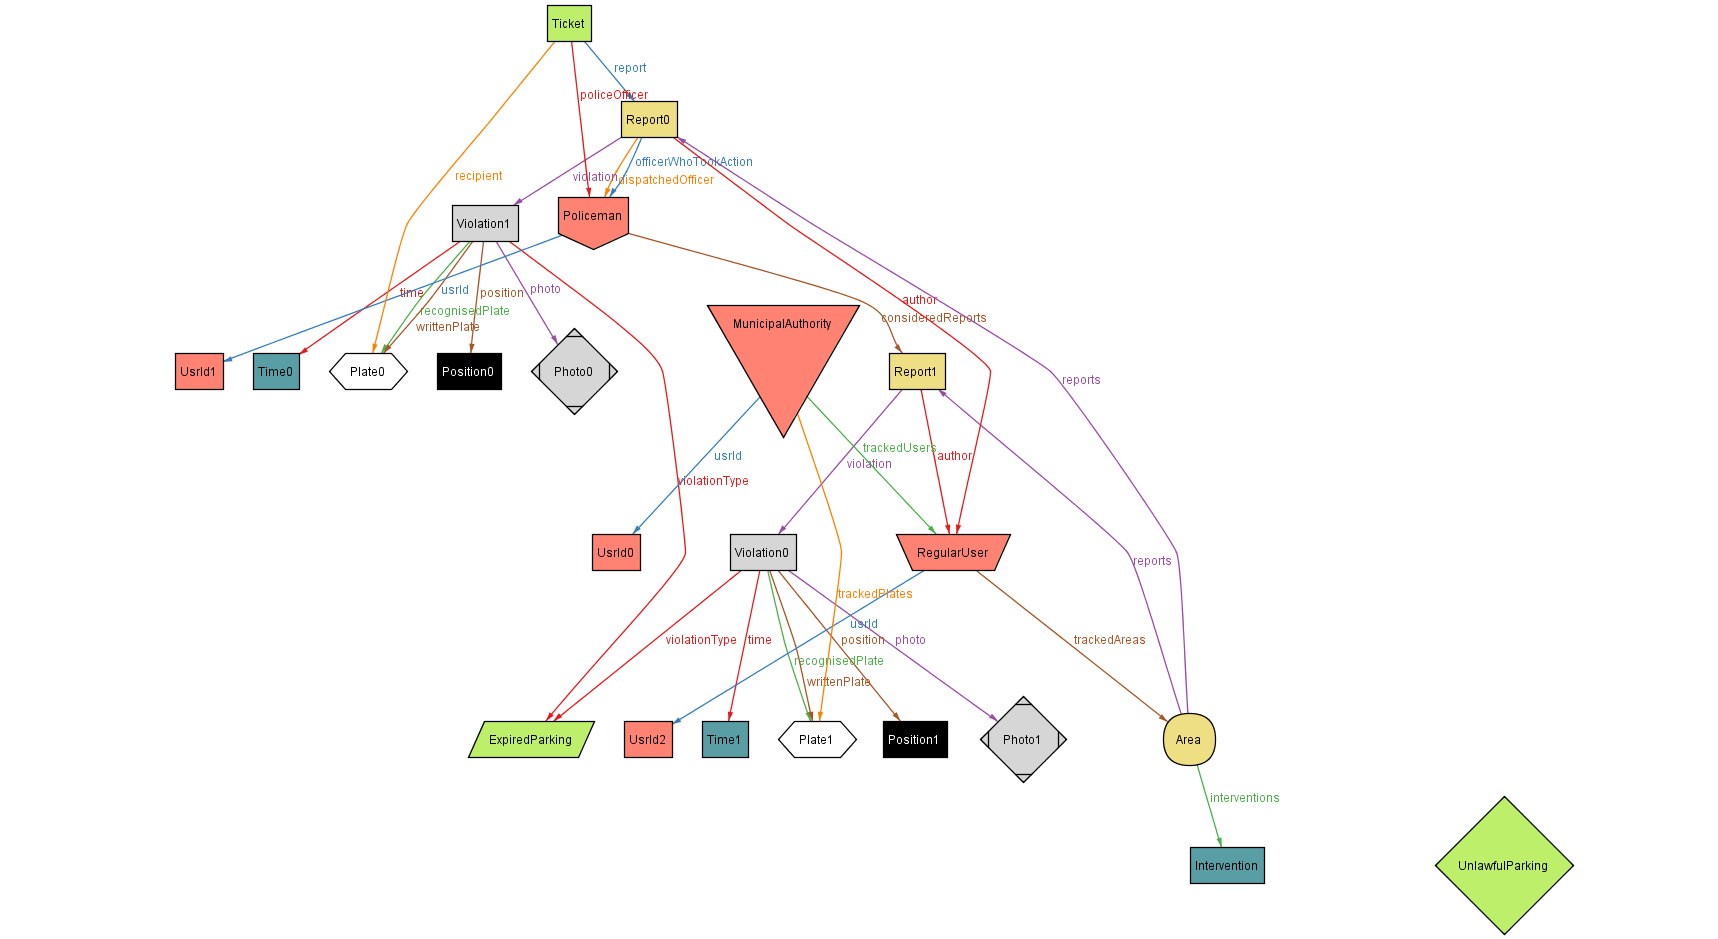
\includegraphics[angle=90, scale=0.35]{Images/world}
	\caption{Example of the world described by the model}
\end{figure}